% Native operation-tree schematic; compile with pdflatex.
% Every bare node has degree three in each displayed graph.
\documentclass[tikz,border=12pt]{standalone}
\usepackage[T1]{fontenc}
\usepackage{lmodern,amsmath}
\usetikzlibrary{arrows.meta,calc}
\definecolor{ink}{HTML}{183444}
\definecolor{blue}{HTML}{1B6780}
\definecolor{amber}{HTML}{AD601A}
\definecolor{pale}{HTML}{F2F6F8}
\begin{document}
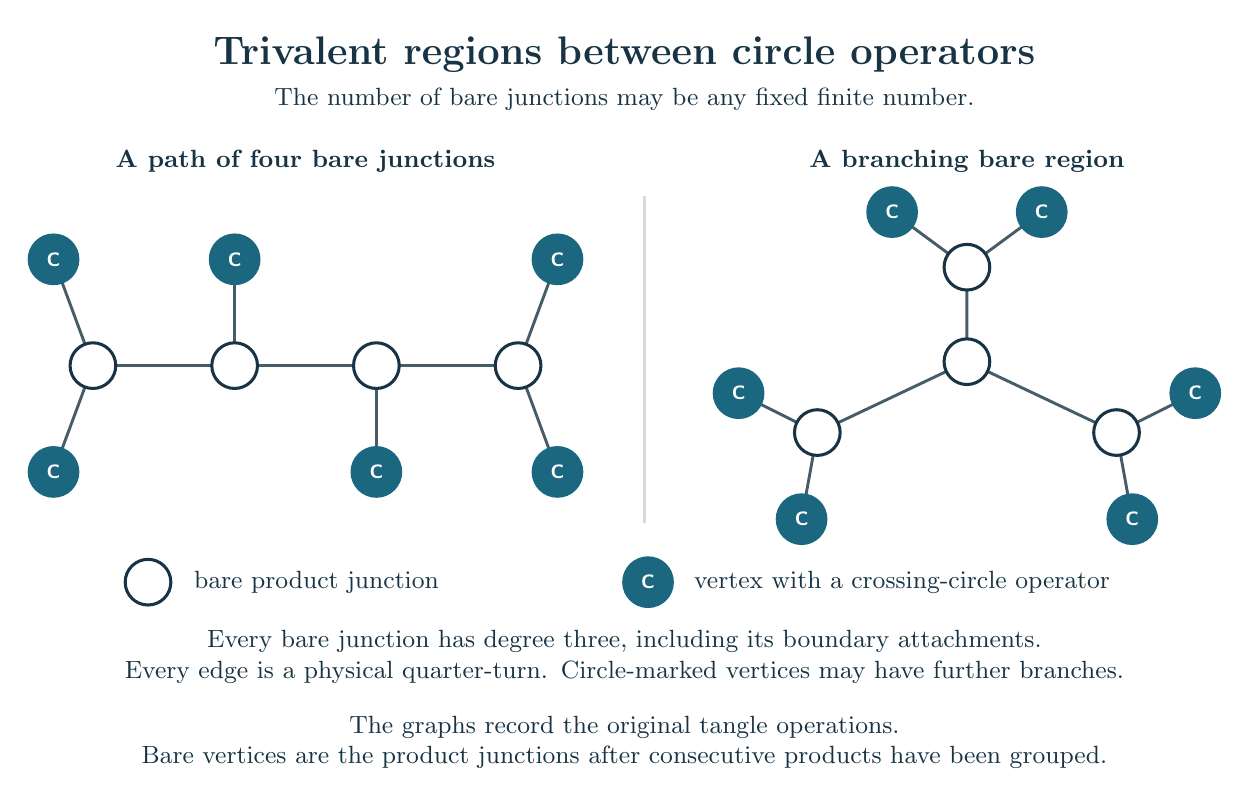
\begin{tikzpicture}[x=1cm,y=1cm,font=\sffamily,text=ink,
  line width=1.05pt,
  bare/.style={circle,draw=ink,fill=white,minimum size=5.8mm,
    inner sep=0pt,line width=1.1pt},
  marked/.style={circle,draw=blue,fill=blue,minimum size=6.2mm,
    inner sep=0pt,text=white,font=\sffamily\scriptsize\bfseries},
  edge/.style={draw=ink!80,line width=1.05pt}]

  \node[font=\Large\bfseries] at (7.25,7.05)
    {Trivalent regions between circle operators};
  \node[font=\small,align=center] at (7.25,6.48)
    {The number of bare junctions may be any fixed finite number.};

  \node[font=\small\bfseries] at (3.2,5.7)
    {A path of four bare junctions};
  \node[font=\small\bfseries] at (11.6,5.7)
    {A branching bare region};

  % First example: four bare nodes and six circle-marked leaves.
  \coordinate (p1) at (.5,3.1);
  \coordinate (p2) at (2.3,3.1);
  \coordinate (p3) at (4.1,3.1);
  \coordinate (p4) at (5.9,3.1);
  \coordinate (pa) at (0,4.45);
  \coordinate (pb) at (0,1.75);
  \coordinate (pc) at (2.3,4.45);
  \coordinate (pd) at (4.1,1.75);
  \coordinate (pe) at (6.4,4.45);
  \coordinate (pf) at (6.4,1.75);
  \draw[edge] (p1)--(p2)--(p3)--(p4);
  \draw[edge] (pa)--(p1)--(pb);
  \draw[edge] (pc)--(p2);
  \draw[edge] (pd)--(p3);
  \draw[edge] (pe)--(p4)--(pf);
  \foreach \v in {p1,p2,p3,p4} \node[bare] at (\v) {};
  \foreach \v in {pa,pb,pc,pd,pe,pf} \node[marked] at (\v) {C};

  % Second example: a three-armed bare tree, again degree three at
  % each bare node, with two marked attachments on each outer node.
  \coordinate (b0) at (11.6,3.15);
  \coordinate (b1) at (11.6,4.35);
  \coordinate (b2) at (9.7,2.25);
  \coordinate (b3) at (13.5,2.25);
  \coordinate (ba) at (10.65,5.05);
  \coordinate (bb) at (12.55,5.05);
  \coordinate (bc) at (8.7,2.75);
  \coordinate (bd) at (9.5,1.15);
  \coordinate (be) at (13.7,1.15);
  \coordinate (bf) at (14.5,2.75);
  \draw[edge] (b1)--(b0)--(b2);
  \draw[edge] (b0)--(b3);
  \draw[edge] (ba)--(b1)--(bb);
  \draw[edge] (bc)--(b2)--(bd);
  \draw[edge] (be)--(b3)--(bf);
  \foreach \v in {b0,b1,b2,b3} \node[bare] at (\v) {};
  \foreach \v in {ba,bb,bc,bd,be,bf} \node[marked] at (\v) {C};

  \draw[ink!18] (7.5,1.1)--(7.5,5.25);
  \node[bare] at (1.2,.35) {};
  \node[anchor=west,font=\small] at (1.65,.35)
    {bare product junction};
  \node[marked] at (7.55,.35) {C};
  \node[anchor=west,font=\small] at (8,.35)
    {vertex with a crossing-circle operator};

  \node[align=center,font=\small,text width=14.8cm] at (7.25,-.6)
    {Every bare junction has degree three, including its boundary attachments.\\
     Every edge is a physical quarter-turn.
     Circle-marked vertices may have further branches.};
  \node[align=center,font=\small,text width=14.8cm] at (7.25,-1.68)
    {The graphs record the original tangle operations.\\
     Bare vertices are the product junctions after consecutive products have been grouped.};
\end{tikzpicture}
\end{document}
